\documentclass[12pt,a4paper]{article}
%\documentclass[fleqn]{scrartcl}
\usepackage[english]{babel}
\usepackage{amsmath}
\usepackage{graphicx}
\usepackage{hyperref}
\usepackage{mathrsfs}  
%\usepackage[colorlinks=true,linkcolor=blue,urlcolor=blue,citecolor=blue,pdfusetitle]{hyperref}
\selectlanguage{english}
\usepackage{mathtools}
\DeclarePairedDelimiter\bra{\langle}{\rvert}
\DeclarePairedDelimiter\ket{\lvert}{\rangle}
\DeclarePairedDelimiterX\braket[2]{\langle}{\rangle}{#1 \delimsize\vert #2}
\usepackage{braket}
\usepackage{appendix}
\usepackage{ amssymb }
\usepackage{amsmath, amsthm}
%\usepackage[backend=biber,style=ieee,citestyle=numeric-comp, url=false, eprint=false, url=true, isbn=false, doi=false]{biblatex}
\usepackage[style=numeric ,citestyle=numeric-comp,backend=bibtex]{biblatex}
\usepackage{graphicx}
%\usepackage{biblatex}
%\usepackage[backend=bibtex]{biblatex}
%\bibliography{library.bib}
\addbibresource{bibli.bib}
\addbibresource{library.bib}
%\makeatletter
%\def\eqref{\@ifstar\@eqref\@@eqref}
%\def\@eqref#1{\textup{\tagform@{\ref*{#1}}}}
%\def\@@eqref#1{\textup{\tagform@{\ref{#1}}}}
%\makeatother 
\begin{document}
\begin{titlepage}
\begin{center}
\begin{figure}[h!]
\centering

\includegraphics[scale=0.3]{Bilder-für-text/uni-basel-logo-ogtag.png} 
\end{figure}

\noindent\rule{\textwidth}{1pt}
\Large\textbf{Fully quantum description of a three level maser, driven by a thermal bath}\\
\noindent\rule{\textwidth}{1pt}
\vspace{0.5cm}
\large{Master-project}\\
%\large{nature12016}\\
\vspace{3cm}
%\normalsize{H. Bernien1, B. Hensen1, W. Pfaff1, G. Koolstra1, M. S. Blok1, L. Robledo1, T. H. Taminiau1, M. Markham2, D. J. Twitchen2,L. Childress3 R.Hanson}\\
\vspace{2cm}

\normalsize{ Sander Stammbach}\\
\normalsize{Prof. Patrick Potts\\Dr. Mateo Brunelli\\ Marcelo Janovitch}\\
\vspace{0.2cm}
12 November 2022\\
\end{center}

\nopagebreak
\vspace{1cm}
\begin{minipage}{.25\textwidth}
 \begin{flushleft}
 \end{flushleft}
\end{minipage}
\hskip.4\textwidth
\begin{minipage}{.25\textwidth}
\end{minipage}
\end{titlepage}
\tableofcontents
\newpage
\section{Introduction}
One of the most important questions in thermodynamics is how to convert
thermal energy into work. For such tasks there exist many classical engines, for
example the steam machines or gasoline engines. %To quantify heat-engines, it's common to look at the ergotropy.
Those ideas also generalize to quantum systems.
In this master-project, a three-level maser, driven by the coupling of a hot and a cold bath is quantified.
The three-level maser is a quantum heat engine (QHE). The work extraction from a classical heat engine is often a moving piston. But in this case
it is a driving field. In the year 1916 Albert Einstein already discussed three ways of
light-matter-interaction (spontaneous emission, absorption, and stimulated
emission)\cite{Li2017}. \\In the paper from  Scovil and Schulz-DuBois 1959 \cite{Scovil1959} investigated whether a laser is a heat engine. In this paper, they toke a maser as a device to transform heat into coherent radiation, because heat can make a population inversion.
In their thermodynamic analysis, they used a single-atom laser. They made a
groundwork for emerging theory of quantum thermodynamics. In practice and also for the calculations, two different reservoirs are necessary. The high-temperature reservoir can be
realized by a fast and accurate
estimation of the thermal occupation of propagating microwave modes  \cite{Scigliuzzo2020}.
\newpage
\section{System and model}
\subsection{3-level-Maser model}
\begin{figure}[h!] 
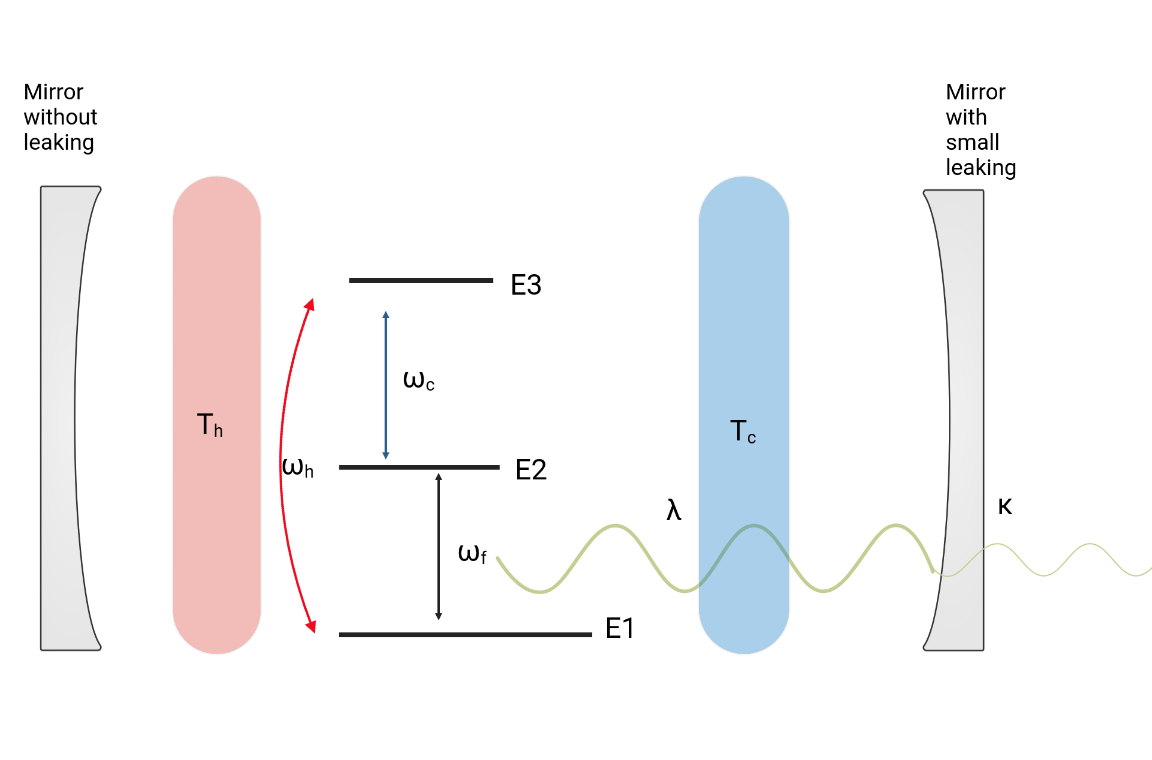
\includegraphics[scale=0.4]{Bilder-für-text/3-Level-System.png}
\caption{Schematic representation of a three-level maser heat engine
continuously coupled to two reservoirs of temperatures $T_h$;  and
$T_c$. The three energy levels are described by $E_1,E_2,E_3$. The
system is interacting with a quantized single mode field. $\lambda$
represents the strength of matter-field coupling. The $\omega_h, \omega_c,  \omega_{cav}$ describes the transition frequencies.}
\end{figure}
A maser/laser consists of two elements. One of them is a gain medium and the other one is an optical resonator. A gain medium is always a material with an atomic transition between two atomic states. When an atom decays from an energetically higher state to an energetically lower state, a photon is created.
In a three level system the three energy levels are $E_1,E_2,E_3$ shown in Fig. 1. In a first part the system gets pumped from the lowest $E_1$ level to the highest level $ E_3$. The resonator should have a longer decay time, so that a population inversion can build up. This means that the system is in the energetically higher state. From this state they come almost exclusively through stimulated emission into the lower state $ E_1$.  The cavity is build of two mirrors. One of the cavity has a small leaking, so that a small part of the photons can leave the cavity. This leaking is quantified by a constant $\kappa$. 
Stimulated emission is a necessary condition for coherent light. Coherent light means all the photons have the same phase and same frequency \cite{Li2017}.
Here we consider that higher level will be reached with a interaction of a hot bath.  
We denote the transition frequencies of $\omega_h=(E_3-E_1)/\hbar$, $\omega_c=(E_2-E_1)/\hbar$ and $\omega_{cav}=(E_2-E_1)/\hbar$.
%Efficiency is defined as $\eta=J/P $
Our cavity is in  resonance, therefore we set $\omega_{cav}=\omega_f$. 
In this three-level system each thermal photon from the bath trigger a lasing photon. 
$J_h$ iast the heat flow from the hot bath, and $J_{cav}$ is the heat flow in the cavity.
The efficiency of the three-level system is then given by the following formula:
\begin{equation}
\frac{J_{cav}}{J_h}=\eta_{maser}=\frac{\omega_{cav}}{\omega_h}<1-\frac{T_c}{T_h}.
\end{equation}

\subsection{Master-Equation} 
An arbitrary state of a cavity and a atom can be described by a total density operator $\hat{\rho}(t)$. %The total density operator can be written in the Hilbert space $ H_ {tot}= H_{system}+H_{bath}$. 
The complete description of the total system's state at a given time $t$ is encoded in this density 
operator $\hat{\rho}$ \cite{Li2017}.
The master equation is:
\begin{equation}
\dot{\rho}(t)=\frac{1}{i \hbar}[H,\rho]+ \mathcal{L}_{h}\rho+ \mathcal{L}_{c}\rho+ \mathcal{L}_{cav}\rho. \label{1}
\end{equation}
To derive the $\hat{\rho}$ we can solve a specific differential equation. This equation is called Lindblad-master-equation \eqref{1}. 
The first part of eq \eqref{1} is the von Neuman equation.%  the analogue of the Schrödinger equation for density matrices.
This part of the equation is unitary and therefore the process is reversible.
$H$ is the the Hamiltonian operator. 
The Hamiltonian describes the energy. 
The field of the laser/maser is composed of three crucial 
parts; the three-level system states, the cavity field, and the interaction between the cavity and the state of the system.
The three-level system and  the  cavity are described in $H_{free}$
The total Hamiltonian,
\begin{equation}
H=H_{free}+H_{int},
\end{equation}
consist of two parts; The part of the free Hamiltonian, where $i$ describe the different states,
\begin{equation}
H_{free}=\sum_{i=1}^3 \hbar \omega_i \ket{i}\bra{i}+\hbar \omega_{cav} a^{\dag}a,\label{2}
\end{equation}
and the interaction Hamiltonian or Jaynes-Cummings Hamiltonian:
\begin{equation}
H_{int}=\hbar g(\sigma_{12}a^{\dag}+\sigma_{21}a).\label{3}
\end{equation}
$g$ is the coupling constant between the system and the photons.  
%The coupling constant is $g$ is given by $\frac{\Omega}{\hbar}$.

The interaction with the various environmental heat baths is described by the non-unitary Liouvillian. $\mathcal{L}_h$ describe the interaction the system and the hot bath, $\mathcal{L}_c$ is the contribution from the interaction with the cold bath coupled with the atom.  $\mathcal{L}_{cav}$ describe the loss of the photons which are in the cavity.  Those $\mathcal{L}_{h,c,cav}$ are also called superoperators, which act on the density operator.  A superoperator is a linear operator acting on a vector space of linear operator. 
The interaction with the various environmental heat baths is described by the Liouvillian:
\begin{equation}
\begin{aligned}
\mathcal{L}_h\hat{\rho}=\frac{\gamma_h}{2}(n(\omega_h,T_h)+1)   \cdot \mathcal{D}[\sigma_{13}]\rho
+\frac{\gamma_h}{2}n(\omega_h,T_h)\cdot \mathcal{D}[\sigma_{31}]\rho \\
\mathcal{L}_c\hat{\rho}=\frac{\gamma_c}{2}(n(\omega_c,T_c)+1)\cdot \mathcal{D}[\sigma_{23}]\rho
+\frac{\gamma_c}{2}n(\omega_c,T_c) \cdot \mathcal{D}[\sigma_{32}]\rho \\
\mathcal{L}_{cav}\hat{\rho}=\kappa((\omega_{cav},T_f)+1)	\cdot\mathcal{D}[a]\rho+
\kappa n(\omega_{cav},T_f)\cdot \mathcal{D}[a^{\dag}]\rho.
\end{aligned}
\end{equation}
$\sigma_{12} $ is the transition operator and defined as $ \sigma_{12}=\ket{1}\bra{2}$. Similar for $\sigma_{13}=\ket{1}\bra{3}, \sigma_{23}=\ket{2}\bra{3}$ . The transition operator describe the transition between one atomic state to a other.
$\mathcal{D}$ is defined with following formula
\begin{equation}
\mathcal{D}[A]\rho=(2A \rho	A^{\dag}-A^{\dag}A\rho-\rho A^{\dag}A).
\end{equation}
Where $A$ represents one of the transition operators $\sigma_{ab}$ or a ladder operator $a$.
The Bose-Einstein occupation number is the mean number of excitations in the reservoir damping the oscillator. It describes the mean occupation number $\langle n(E) \rangle$ of a quantum state of energy $E$, in thermodynamic equilibrium at absolute temperature $T $ for identical bosons as occupying particles.$ n$ depends on the temperature and the frequency.
$n$ is defined as:
$
n_i(\omega_i,T)=\frac{1}{\exp[\frac{\hbar \omega_i}{k_b T_i}]-1}.
$
$\kappa$ describes the rate of photons which leave the cavity.
The  prefactor $\gamma_c ,\gamma_h$ describes the spontaneous decay rates. We set $\gamma_c ,\gamma_h  =\gamma=1$ in this calculation and express also $\kappa$  and $\omega_i$ in  therms of  $\gamma$.
In this case the master equation is solved for the steady states.
A steady state is a state or condition of a system or process, that the density matrix of the state does not change in time, or the changes are negligibly. Therefore all observables do not change in time either. 
It contains the whole description of the three-level system and the cavity.
\section{Methods}

\subsection{Implementation of the three-level-system in qutip}
The master equation is solved numerically. For that it is necessary to define the constants first.
In our case, only the transition between $\ket{1}$ and $\ket{2}$ interact with the light. 
%The constants $\hbar $ and the Boltzmann factor $k_B$ are 1.
Defined as constants are the three different Bose-Einstein occupation $n_h$, $n_c$ and $n_f$
The transition-operators $\sigma_{ab}$ are  made by qutip \cite{Nation2022} implementation of the tensor product of $\ket{a}\bra{b}$ and the identity matrices of size of maximum photon number. 
%In the same way, I implemented the other transition operators and 
$\ket{1}$ and $\ket{2}$ are basis states. For our purpose, it will  always suffice to truncate the photon's Hilbert space at $n=29$. So we get  90 x 90 matrices. 
The projectors are implemented similarly, with the matrix $\ket{a}\bra{a}$
With those it is easy to construct the Hamiltonions, $H_{free}$ and $H_{int}$, as in Eq. \eqref{2} , Eq .\eqref{3}.
To calculate the the density matrices for steady states we can also use a qutip function.
This function needs the total Hamiltonian and a list of the non-unitary operators as arguments.
%We can we can construct this list as a multiplication of our transition-operators and the tree different Bose Einstein occupation numbers times the different $\gamma$-factors. 
As output of the function steady-state we get the density-matrices for steady-states. \cite{Nation2022}
\section{Lasing transition}

\subsection{Wigner function and phase-averaged coherent states}
The output of a laser is coherent light.
The quantum description of coherent light is a coherent state. The photon number distribution of coherent light is a Poisson distribution.
In our case the output is a phase-averaged coherent state (PHAV). 
Thats a coherent state which has a averaged phase $\phi$ around $2\pi$.
Randomizing the phase of a coherent state doesn't change the photon-number distribution. \\

A Wigner function is a representation of a general quantum state of light \cite{Allevi2013}.
The function describes the probability density in phase space.
\begin{equation}
w(x,p)=\frac{1}{2\pi \hbar}\int_{- \infty}^{\infty} d\xi e^{\frac{-i p \xi}{\hbar}}\bra{x+\frac{1}{2}\xi}\rho\ket{x-\frac{1}{2}\xi}.\label{4}
\end{equation}
%The Wigner function from a coherent state is a Gaussian. 
The Wigner function of a coherent and a phase-average-state is non-Gaussian, because of Eq. \eqref{4}  is a  not a Gaussian. 
 So we get a new term of $\exp(i\pi\phi)$ in it. 
The standard coherent state $\ket{\alpha}$ can be represented by following formula: 
\begin{equation}
\ket{\alpha}=e^{\frac{-|\alpha|^2}{2}}\sum_{n=0}^{\infty}\frac{|\alpha|^n e^{in\phi}}{\sqrt{n!}} \ket{n}.
\end{equation}
The PHAV state will be obtained by integrating over the phase $\phi$.
\begin{equation}
\rho_{PHAV}=\int_0 ^{2\pi}\frac{d\phi}{2\pi}\ket{\alpha(\phi)}\bra{\alpha(\phi)}=\sum_{n=0}^{\infty}p_{nn}\ket{n}\bra{n},\label{22}
\end{equation}
thus is equal to
\begin{equation}
\rho_{PHAV}= \sum_{n=0}^{\infty}\exp(-|\alpha|^2)\frac{|\alpha|^{2n}}{n!} \ket{n}\bra{n}.\label{11}
\end{equation}
Eq. \eqref{11} is implemented in python to visualize a photon number distribution and Wigner plot  Eq \eqref{4}, shown in Fig 2.
A Fock plot shows the occupation probability $p_{nn}$.
So the goal of this work is to find a $n_h$ which yield a PHAV state,
as in \cite{Allevi2013} 
For the Wigner function \eqref{4} we finally get the following equation
\begin{equation}
w(x,p)=2  \exp\bigl[-2\bigl(|\alpha|^2+|x+ip|^2\bigr)\bigr) I_0 (4|\alpha| |x+ip|).
\end{equation}
$I_0$ is the first  Bessel function.
This function is plotted in Fig. 2
\begin{figure}[hbtp]
\hspace{-1.4cm}
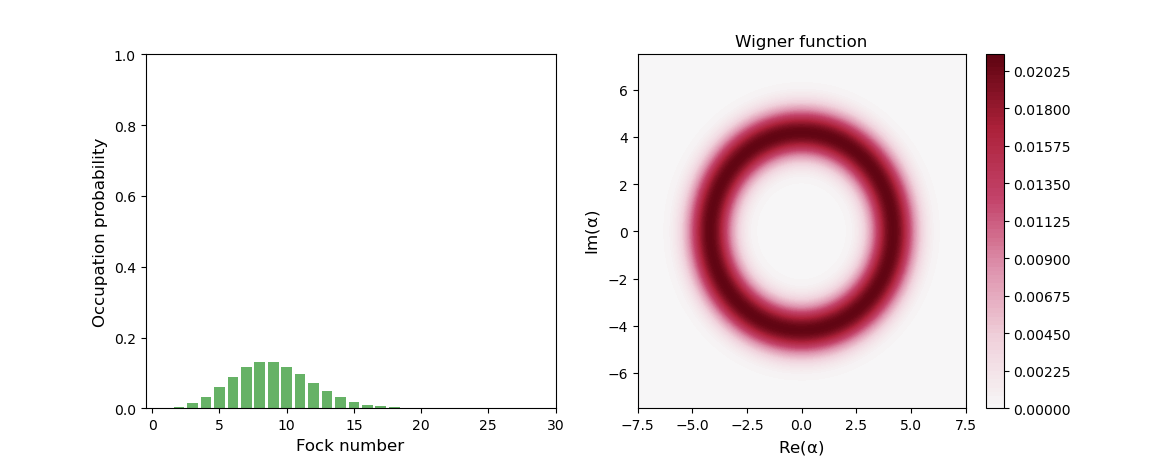
\includegraphics[scale=0.55]{Bilder-für-text/PHAV-rho.png}\label{21}
\caption{The photon number distribution, also called Fock plot of the density matrix of $\rho_{PHAV}$ with the parameter $\alpha=3.5$, is shown in Fig. 2 at the left side. At The right side is the Wigner function illustrated.}
\end{figure}


\newpage
\subsection{Double threshold behaviour and population inversion}
 When we work with density matrices, it is common to work with expectation values with $\langle A \rangle=Tr[A\cdot\rho]$.
 $A$ is an operator and describe a measurement.
With this, we can calculate the expectation value from an Operator. 
The population inversion is seen by calculating the probability for the levels number ($Tr[\ket{i}\bra{i} \rho]$) and i stands for the different occupation of the state. Fig. 3a.  With high $n_h$ the probability for the system to stay in a the state $\ket{2}$ increases as well. If $P2>P1$, we speak about a population inversion.  
%All the simulation are done with steady states.
Lasing starts once a threshold for emission is attained, however, increasing the heat flow too much will end up producing  thermal light instead of lasing. This phenomena is called a double threshold behaviour \cite{Li2017}. To investigate this double threshold behaviour, we study the steady states of a three-level system.
This double threshold behaviour can can be explained by the Zeno effect. 
The Zeno effect describes that the transition from one state to the other can be stopped by rapid successive measurements. 
The system behaves similarly when sufficient stimulation is applied quickly. 
With the plot  $Tr[n\rho] =\langle n\rangle$ against different $n_h$ Fig. 3b we see this double threshold behaviour because, when the hot bath temperature $n_h$ is too low $(n_h \approx n_c)$ we have also a  low photon number. With increasing $n_h$, population inversion happens, the photon number increase and the output looks like a PHAV state,  see  Fig. 2. With too high $n_h$ the average photon number decreases again and this system shows a double threshold behaviour, the excitation is too weak, and we say that the system is below the lasing threshold with the output light of a thermal state.
\begin{figure}[h!]
\hspace{-1cm}
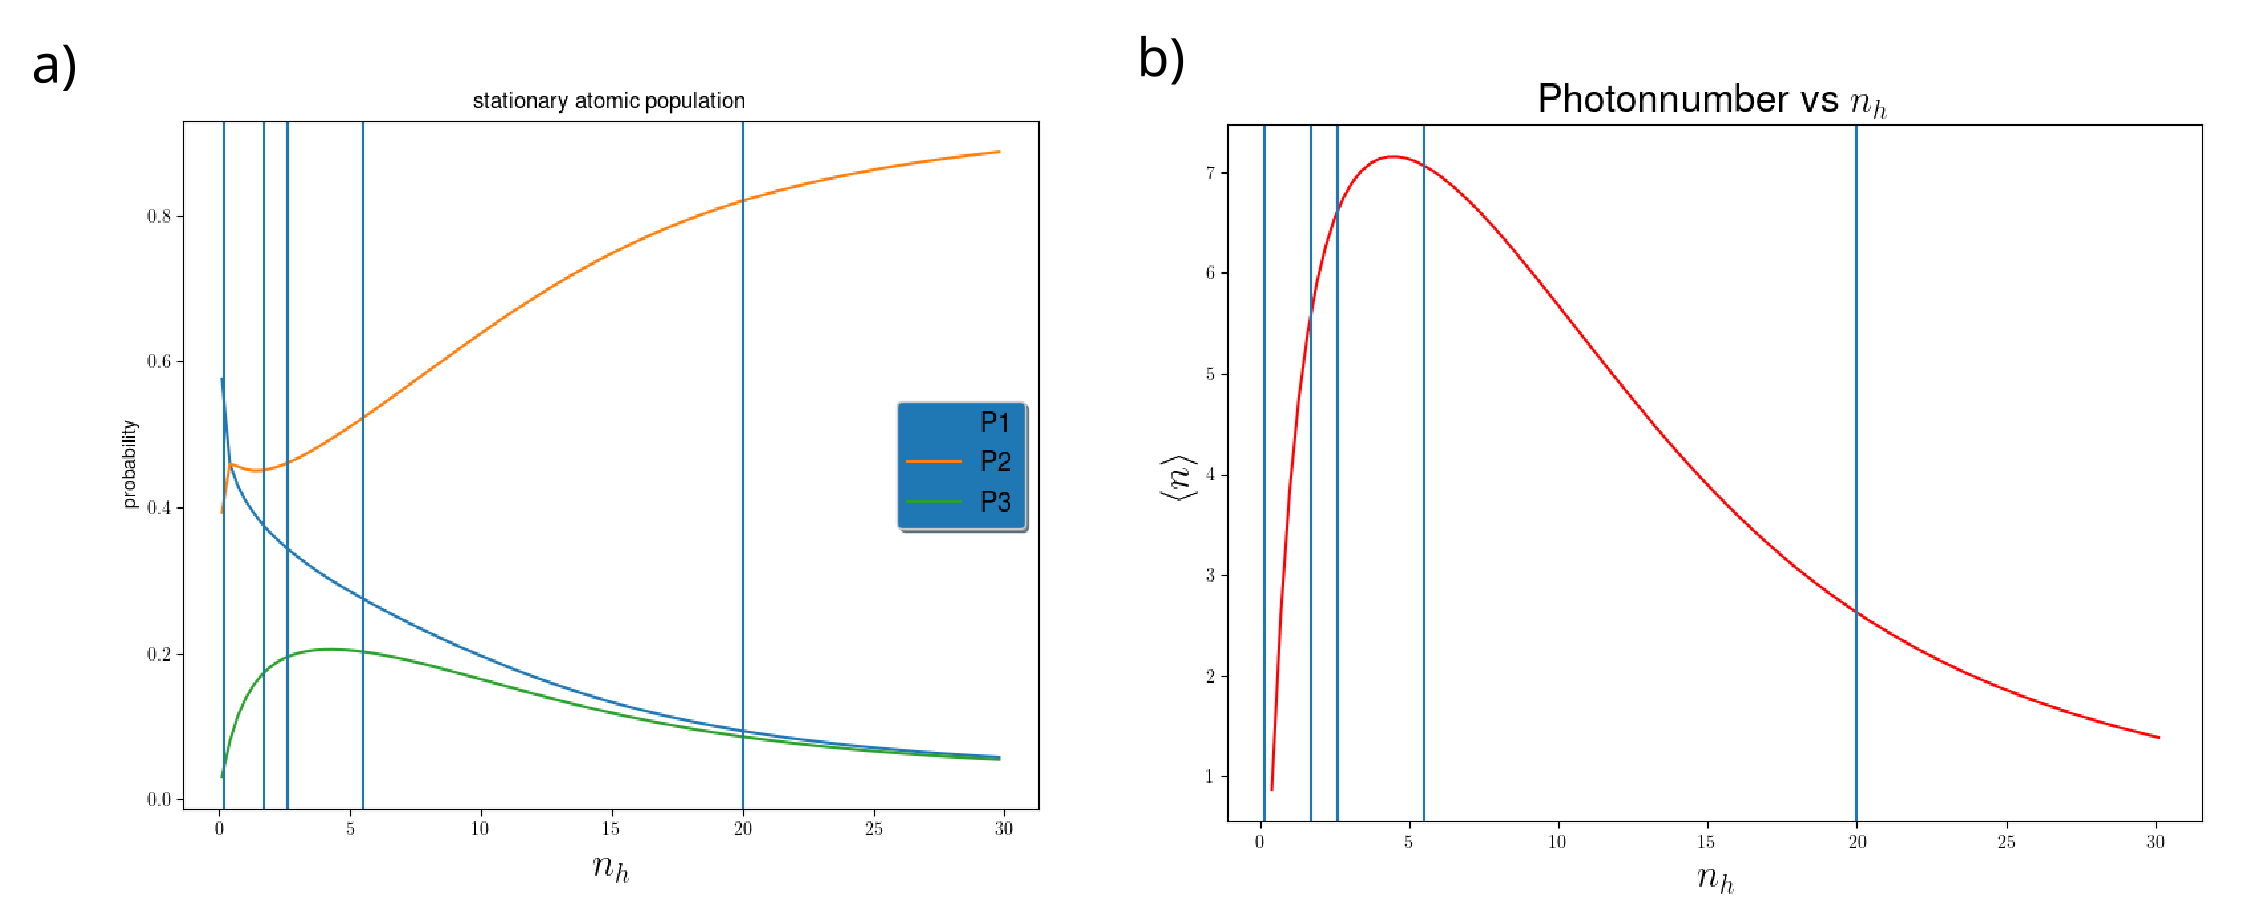
\includegraphics[scale=0.2]{Bilder-für-text/Energy_1.png}
\caption{In Fig. 3a the probability for an atom to stay in a state $\ket{1}, \ket{2}$ or $\ket{3}$ vs $n_h$is plotted. With a increasing $n_h$ $P2$ increase as well until a population inversion happens $P2>P1$. The probability for $P1,P2,P3$ is in the region of $n_h=5 $ well distributed. The parameters for the first plot are $n_c=0.02 ,n_f=0.02,\kappa=0.01\gamma_h $. The blue lines mark the values of $ n_h$ for which the Wigner functions are plotted. In Fig. 3b we see, the expectation value of the photon number versus $n_h$.}
\end{figure}
\newpage
An other way to see the double threshold behaviour of the system is to analyse the Wigner function plot. For that the reduce density matrix $\rho_{free}$ will be used to make Wigner and Fock plots numerically. For the calculation of the coherent state, the information about the system state is not necessary and the system gets traced out. 
It is possible to make the partial trace of $\rho$, to trace out the reduced density matrices $\rho_{free}$. 
The first result are plots from the photon number distribution and the Wigner function.
  %$\hbar$ and $kb$ equal to one.
 For all calculations, I set the parameters $\gamma_h, \gamma_c $ are set to $\gamma=1$. And $\kappa=0.028 \gamma_h$
I calculated Wigner functions for this set of parameters, shown in Fig. 4 and Fig. 5.\\
Those rings which are shown in Fig. 4 and Fig. 5, are similar to the plot of Fig. 2.
If we have a small $\kappa$ means less photons will leave and stay in the cavity. we see that in the plot of the photon number distribution.
In the first plot I set a high leaking-parameter $\kappa=1 \gamma_h$. Shown in Fig. 4.
This means that many photons leave the cavity, and only a few remain in the cavity. 
We see, that the occupation-number the photon number distribution is most zero and the probability for one photon is just 0.1.

\begin{figure}[hbtp]
\centering
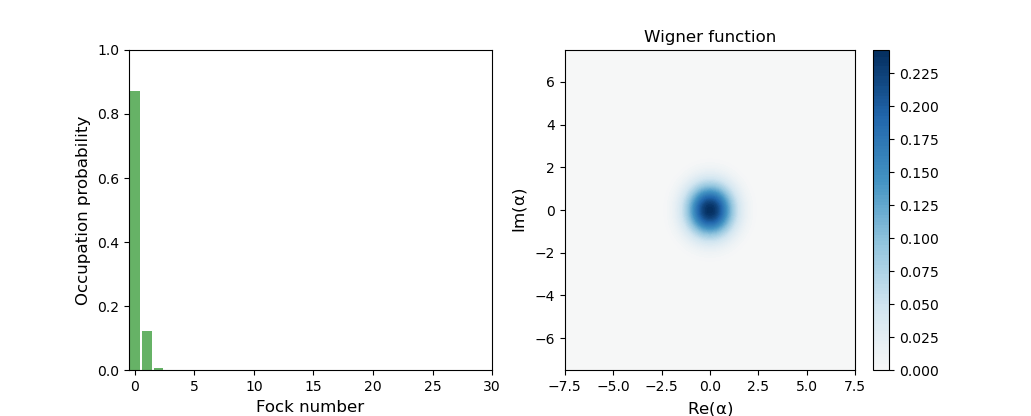
\includegraphics[scale=0.55]{Bilder-für-text/Figure_1.png}
\caption{The parameters for the first plot are $n_h=2.6, n_c=0.001, n_f=0.02, \kappa=1\gamma $. With  the factor of $\kappa=1\gamma_h$ the leaking is too high for a lasing state.}
\end{figure}\newpage

In the plots of Fig 5 I took the same parameters again, but with a lower $\kappa$. We get more photons in the cavity. We see the distribution in the photon number distribution plot and a PHAV state in the Wigner function. 
\begin{figure}[h!]
\centering
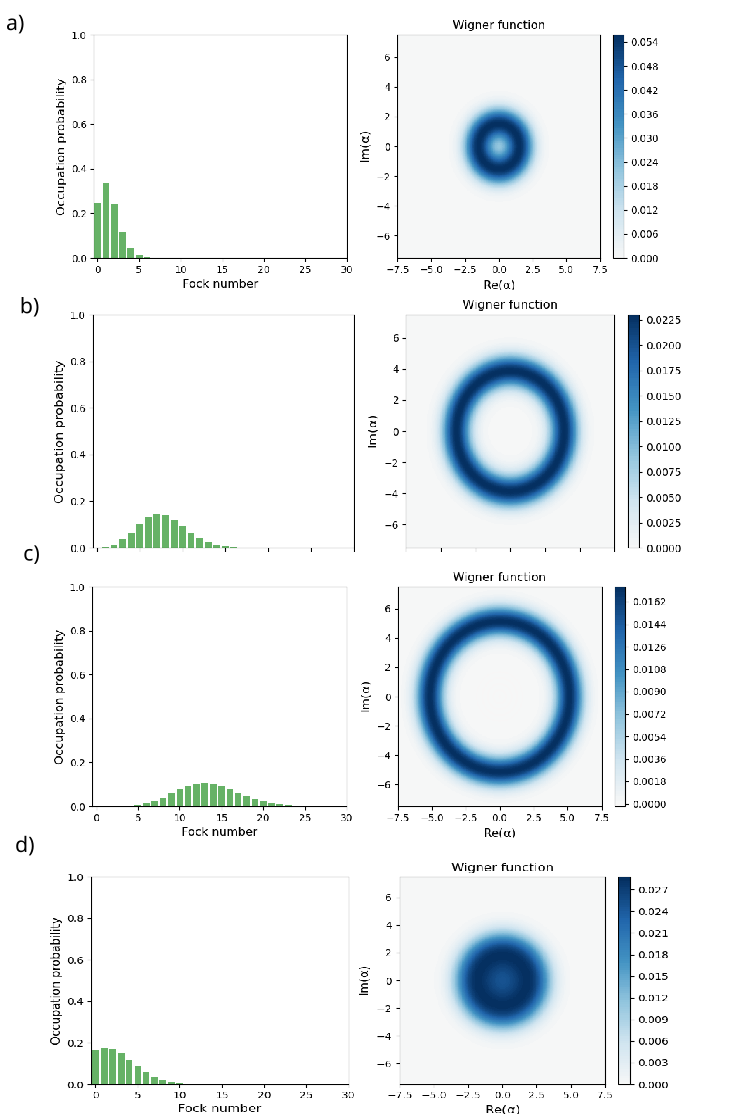
\includegraphics[scale=0.55]{Bilder-für-text/4-fits2.png}
\caption{For all of the four the parameters are $n_c=0.001, n_f=0.02, \kappa=0.1\gamma$. Cavity with a small leaking.
\textbf{a)}The parameters for $n_h$ are $n_h=0.2 $.
\textbf{b)}$ n_h=2.6$ 
\textbf{c)} $ n_h=5.5$ 
\textbf{d)}$ n_h=20$. 
\textbf{4b,4c}looks similar to a PHAV state from Fig 2. The blue lines from Fig 4 mark the values of $n_h$ where the plots from Fig 4 are done for. }
\end{figure}
\newpage
We see in Fig 5a that start to get a state which looks like PHAV state.
If we increase  $2n_h $,
then the cavity photon number increases again when increasing $n_h$ at the
high temperature regime, as shown in Fig. 5b, Fig 5c. 
If we further increase  $n_h >10$, we see the double threshold behavior. 
The state of Fig. 5d is done in a very high temperature region with the value of $n_h=20$. In this  case the output is a similar to a thermal state, so no PHAV state anymore and the output is below the threshold.
%(Dieser Abschnitt ist zum teil übernommen und muss noch umgeeschrieben werden)
\section{Thermodynamics}
\subsection{Heat currents}
The first law of Thermodynamics says: "The change in internal energy of a closed system is equal to the sum of the change in heat and the change in work."
That is  equal to the equation
\begin{equation}
\Delta U=\Delta Q+\Delta W.
\end{equation}
In quantum mechanics  the equation can be  rewritten as
\begin{equation}
\frac{d\langle H \rangle}{dt}=Tr[H_{free} \cdot \mathcal{L}[\rho]]]+Tr[\partial_t H \rho]. \label{d}
\end{equation}
In the case of this calculation with steady states $\Delta U$ or $\frac{d\langle H \rangle}{dt}$ is zero. $\Delta W$ is also zero. This can be justified because $\partial_t H=0 $ and therefore the the first law says that $\langle J_{tot} \rangle$ have to be zero.
To calculate the average heat flow we can take the trace from $Tr[H_{frre}\cdot \mathcal{L}[\rho]]$. 
\begin{equation}
\langle J_{tot}\rangle=Tr[H_{free}\cdot \mathcal{L}_h[\rho]]+Tr[H_{free}\cdot \mathcal{L}_c[\rho]]+Tr[H_{free}\cdot \mathcal{L}_{cav}[\rho]].\label{13}
\end{equation}
A part of my work is to calculate the occupation probability of the states analytically. 
The calculation is made in two steps. For the hot and the cold bath, we have a transition-operators in the trace.
%The trick of this calculation is, to get the form $Tr[\sigma_{ab}\rho \sigma_{ab}^{\dag{}}]$.
% because this corresponds to the probability that the system is in state b $(Pb)$
The equation gave the following result:
\begin{equation}
\langle J_h \rangle=Tr[H_{free}\cdot \mathcal{L}_h[\rho]]=\hbar \omega_h \gamma_h (2n_h+1) ( P1-P3) ,\label{a}
\end{equation}
The same calculation can be done for the interaction with the cold bath.
\begin{equation}
\langle J_c \rangle=Tr[H_{free}\cdot \mathcal{L}_c[\rho]]=\hbar \omega_c \gamma_c (2n_c+1) ( P2-P3) ,\label{b}
\end{equation}
For the calculation the $Tr[H_{free}\cdot \mathcal{L}_{cav}]$, I get the following result
\begin{equation}
\langle J_{cav}\rangle=T[H_{free}\cdot \mathcal{L}_{cav}[\rho]]=2\hbar \omega_{cav}\kappa (n_f-\langle a^{\dag{}}a \rangle).\label{c}
\end{equation}
$J_h$ is a energy input in the system, therefore it has a other signe as $J_c, J_{cav}$.
The calculations are shown in Fig. 8 and Fig. 9 in the Appendix.
With the density matrix it is possible to calculate the heat flux by taking $Tr[H\cdot \mathcal{L}\rho]$. 
and plot this for different  $g$. 
%In the second step of the calculation we look for $ \langle J_{tot}\rangle$ on different coupling constants $g$.
%In other words, in the plot below, the Trace from the density matrices times the Liouvilian against the coupling constant is visualized.
%The master equation depends on three different Liovillien therms.
 I calculated the expected heat flows depends on he cold, the hot bath and the interaction with the cavity are shown in Fig.  6.
%Fig. 6 shows  for the parameters $n_h=2.6, n_c=n_{f}=0.02\gamma,\kappa=0.01\gamma$ is shown below.

\begin{figure}[hbtp]
\centering
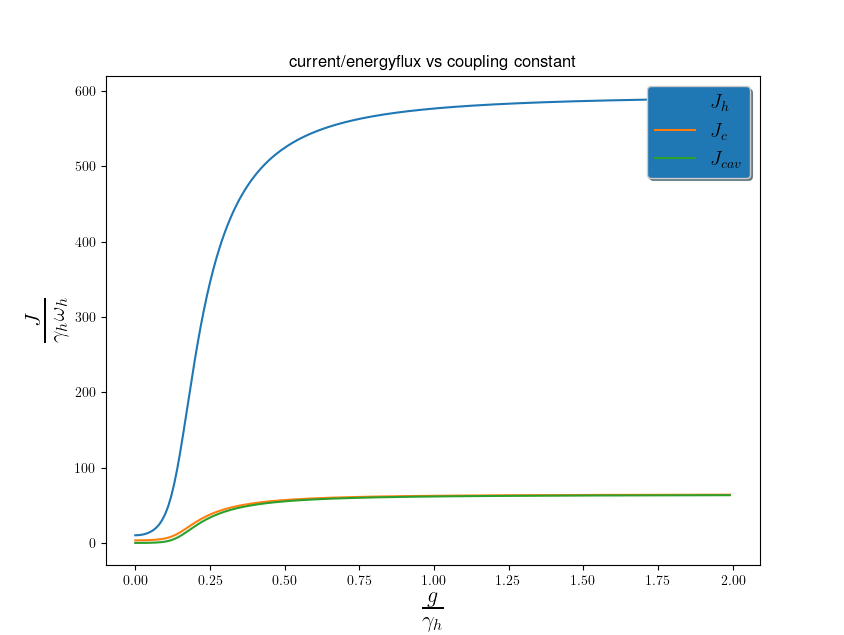
\includegraphics[scale=0.6]{Bilder-für-text/Energie_1.png}
\caption{Energy flux vs g with the parameters The parameters for the plot are $ n_h=2.6, n_c= n_f=0.02,\kappa=0.01\gamma $.  For the for the frequencies $\omega_f=30\gamma,\omega_h=150\gamma, \omega_c=120\gamma$ are used. }
\end{figure}
\subsection{Entropy production}
Another relevant concept is the entropy. It is also a physical property which is described by the following equation.  
\begin{equation}
\Delta S = \sigma-\frac{Q}{T}
\end{equation} 
the second law of thermodynamics says that, for a isolated system, the entropy always remains the same or increases, but never becomes smaller. In terms of instantaneous quantities, this principle can be expressed by the entropy production rate $\dot \sigma$, which should always be larger or equal than zero.
\begin{equation}
\dot{\sigma}\geq 0
\end{equation}
%Entropy is defined it as the quotient of an infinitesimal amount of heat $\Delta Q_{rev}$to the instantaneous temperature.
%\begin{equation}
%\Delta S = \frac{Q}{T}
%\end{equation} 
Since we are interested in steady-state quantities, it is possible to calculate the entropy production rate as the sums of the heat flow contributions \eqref{a}-\eqref{c} divided by the respective bath temperature \eqref{d}.
The entropy production rate for steady state is then given by the formula
\begin{equation}
 \dot{\sigma} =\frac{J_c}{T(n_c)}+\frac{J_h}{T(n_h)}+\frac{J_{cav}}{T(n_{cav})}.\label{666}
 \end{equation}
The entropy production rate for different $n_h$ is plotted in Fig. 7. We see a clear maximum at the value of $n_h \approx 5$.  The contribution to the entropy production rate from the hot bath is less than the contribution from the cold bath, this is because the temperature of the hot bath is much higher, and therefore $\sigma=\frac{J_h}{T}$ is smaller than the entropy production rate of the cold bath. 
We also see that the plot of  the entropy production rate resembles that of the average  photon number Fig. 3.
The blue lines in Fig. 5 mark the values of $ n_h$ for which the Wigner functions are plotted. In Fig. 3b we see, the expectation value of the photon number versus $n_h$. When we compare the lasing output Fig. 5 with the entropy, we see that the lasing output is a PHAV state, when the entropy production rate is high. 
If $n_h$ is large, the coupling with the hot bath dominates with respect to the coupling to the cold bath and to the photons leaking outside the cavity. The larger $n_h$, the closer the system gets to be an equilibrium state with the hot bath. That's why the entropy production rates decreases for large  $n_h$. As consequence we get a PHAV state as laising output again.

\begin{figure}[hbtp]
\centering
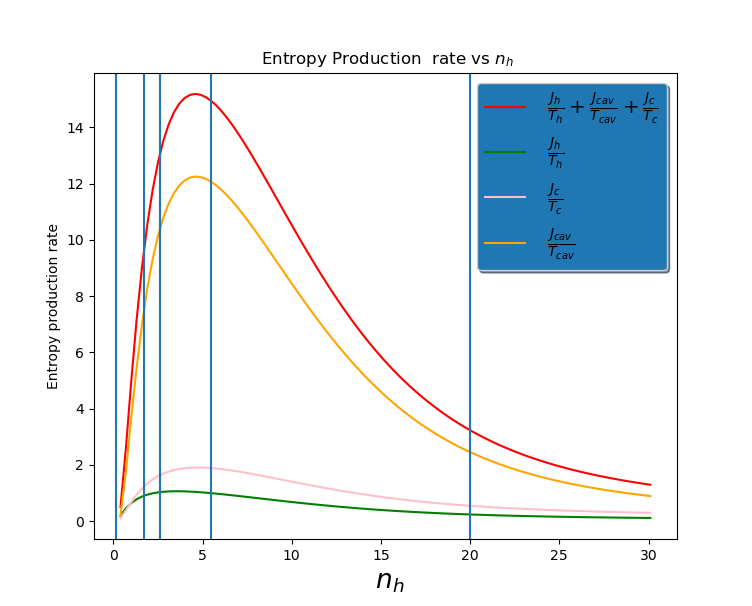
\includegraphics[scale=0.6]{Bilder-für-text/Entropy}
\caption{The entropy production for different $n_h$. The parameters for the first plot are $n_c=0.001, n_f=0.02,\kappa=1\gamma$. As in paper \cite{Li2017} is used the values for the frequencies $\omega_f=30\gamma,\omega_h=150\gamma, \omega_c=120\gamma$.}
\end{figure}
\newpage
\section{Conclusion and outlook}
In those numerical calculations are found states which  look similar to PHAV states, driven by the coupling of two different thermal bath. We found the double threshold behavior from the system, by calculating different energy flux for different $n_h$. As in the paper \cite{Li2017}.
With the condition that $n_c, n_{cav}$ is almost zero, the leaking $\kappa$ is small too, and the hot bath received a value between 1 and 5.5. When we compare the Winger functions of the numerical calculated states from a our three-level system Fig 5b,5c with the Wigner plot of a PHAV state Fig. 2, we see, that they are pretty similar. As conclusion; it's possible to get a phase average coherent state. 
In Fig. 6 we see the average of the current, calculated with the formula Eq. \eqref{13} for different coupling constants $g$.
The conclusion from Fig. 6 is, that the current increase at most between the $ 0<g<0.25$.
In Fig. 5a we see the probability in which state the  system is. If we increase the temperature from the hot bath, we see that the occupation probability of $P2$ increase as well. A  population  inversion is visible.
Fig. 3 helps to get some conclusion about the system starts lasing and when it stops. With a too small temperature, it has not enough energy in the system and the photon number is low Fig 5a. If $n_h$ increase more, a maximum lasing output is reached  Fig 5b,5c. If the temperature increasing further, the system is in the highest level, therefore the Rabi oscillation between $E_0$ and $E_2$ does not exist anymore and we get a thermal state Fig 5d.
At higher heat of the warm bath, dephasing of the system occurs. Thus, it interacts more with the environment. This has the same effect as if the system is measured often. The Zeno effect then make that the system no longer oscillates between two different states. 
%Spontaneous  emission could be a problem too, that the photons which leave the atoms are not in a coherent state anymore.
The consistent numerical and theoretical results we have obtained in the characterization of both PHAV states.
%A motivation to get those PHAV states is; with two PHAV states reinforce the
%possibility of using them for applications to communication protocols \cite{Allevi2013}.
In further calculation  we will look at the thermodynamic uncertainty relation (TUR) and a second laser as input.
%\section{References}
%\bibliographystyle{plain}
\printbibliography



\newpage
\section{Appendix}
The hole Master equation without any substitution:
\begin{equation}
\mathcal{L}\hat{\rho}=\frac{\gamma_h}{2}\biggl[  \frac{1}{\exp[\frac{\hbar \omega_h}{k_b T_h}]-1}+1   \biggr]\cdot \biggl(2 \sigma_{13}\cdot\rho\cdot \sigma_{13}^{\dag}-\sigma_{13}^{\dag}\sigma_{13}\rho-\rho\sigma_{13}^{\dag}\sigma_{13}\biggr) $$\\$$
+\frac{\gamma_h}{2}\bigg[  \frac{1}{\exp[\frac{\hbar \omega_h}{k_b T_H}]-1}\biggr] \cdot\biggl( 2 \sigma_{31}\cdot\rho\cdot \sigma_{31}^{\dag} -\sigma_{31}^{\dag}\sigma_{31}\rho-\rho\sigma_{31}^{\dag}\sigma_{31}\biggr)$$\\$$
+\frac{\gamma_c}{2}\biggl[  \frac{1}{\exp[\frac{\hbar \omega_c}{k_b T_c}]-1}+1   \biggr]\cdot \biggl(2 \sigma_{23}\cdot\rho\cdot \sigma_{23}^{\dag}-\delta_{23}^{\dag}\sigma_{23}\rho-\rho\sigma_{23}^{\dag}\sigma_{23}\biggr)$$\\$$
+\frac{\gamma_c}{2}\bigg[  \frac{1}{\exp[\frac{\hbar \omega_c}{k_b T_c}]-1}\biggr]
\cdot\biggl( 2 \sigma_{32}\cdot\rho\cdot \sigma_{32}^{\dag}-\sigma_{32}^{\dag}\sigma_{32}\rho-\rho\sigma_{32}^{\dag}\sigma_{32} \biggr)$$\\$$
+\kappa\biggl[ \frac{1}{\exp[\frac{\hbar w_f}{k_b T_f}]-1}+1\biggr] \cdot\biggl( 2 a\rho a^{\dag} -a^{\dag}a\rho-\rho a^{\dag}a\biggr)$$\\$$
+\kappa\biggl[ \frac{1}{\exp[\frac{\hbar w_f}{k_b T_f}]-1}\biggr]\cdot \biggl(2 a^{\dag}\rho a -aa^{\dag}\rho-\rho a a^{\dag}\biggr)$$\\$$
\end{equation}


\begin{figure}[hbtp]
\centering
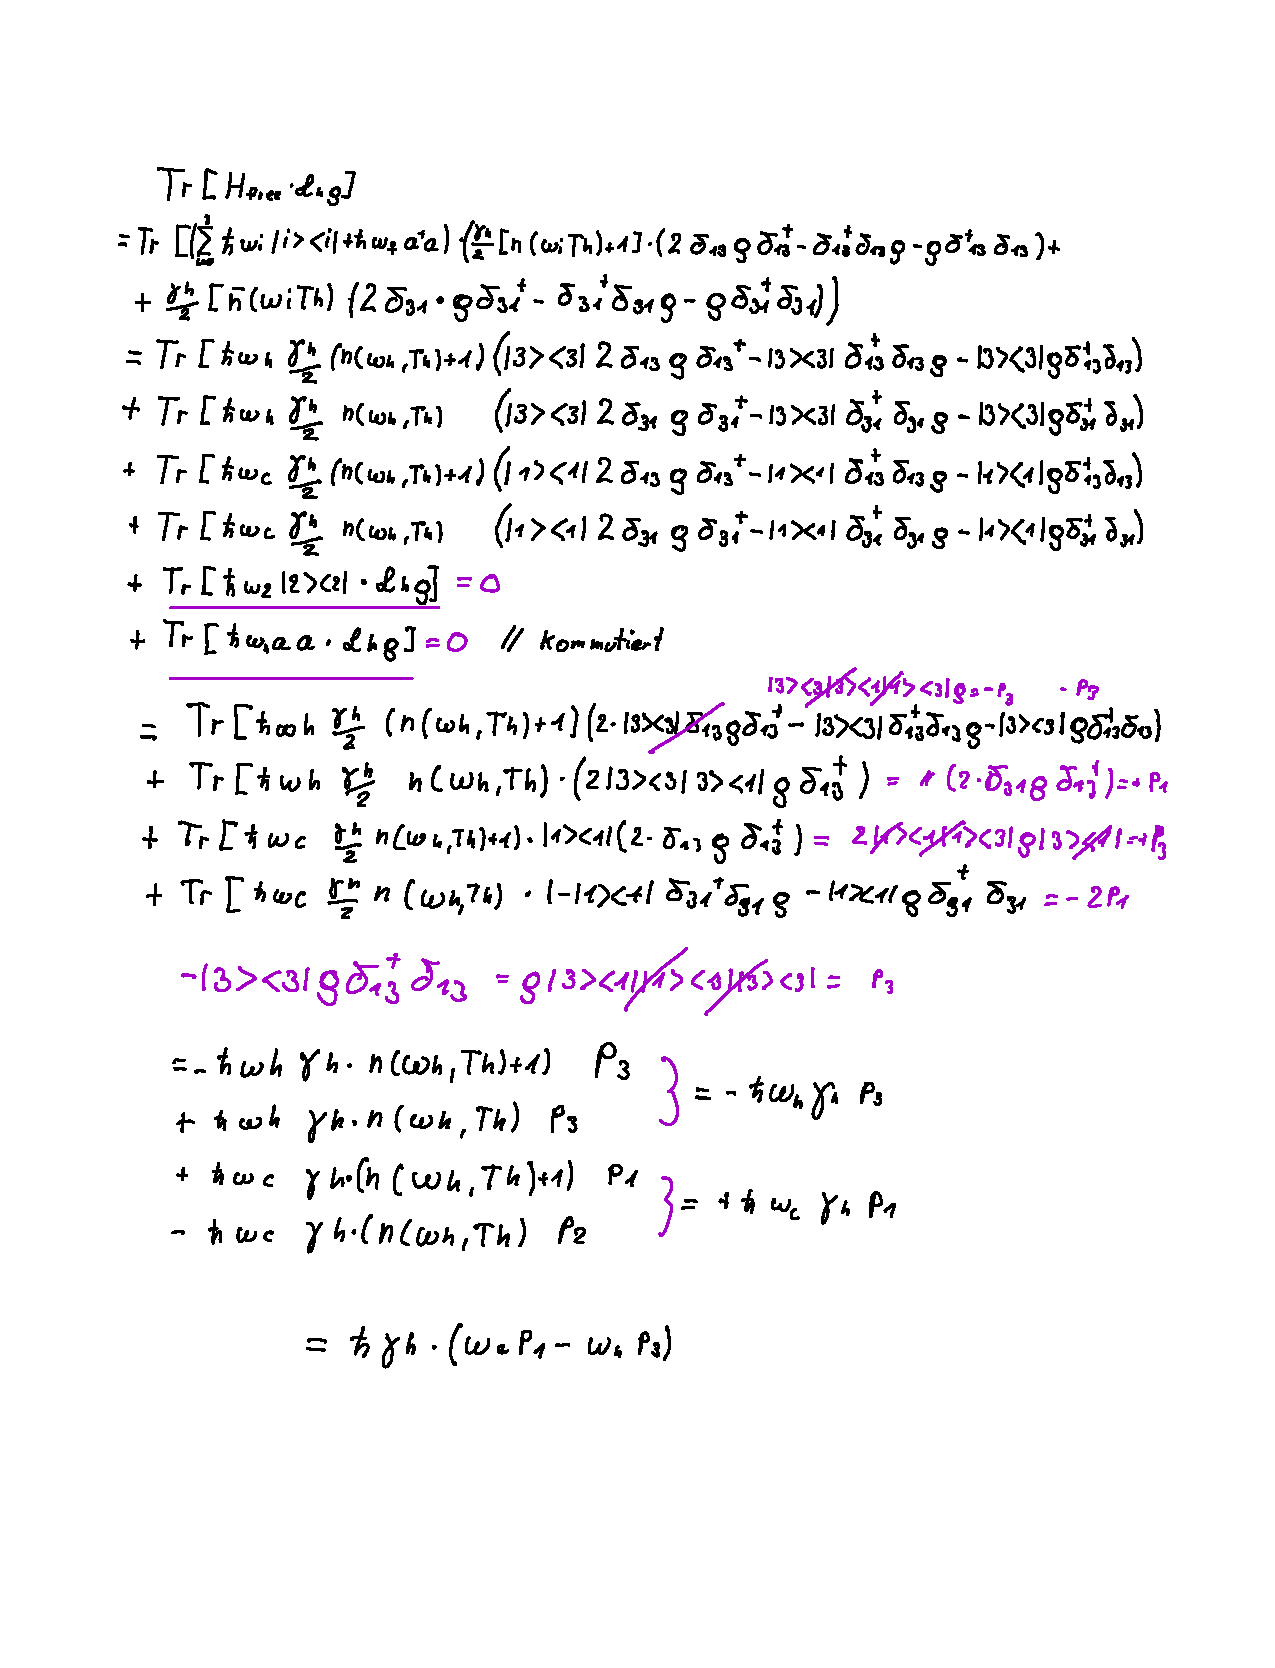
\includegraphics[scale=0.5]{Bilder-für-text/Berechnung-Tr[HL].pdf}
\caption{Calculation for $Tr[H \mathcal{L}]$.}
\end{figure}

\begin{figure}[hbtp]
\centering
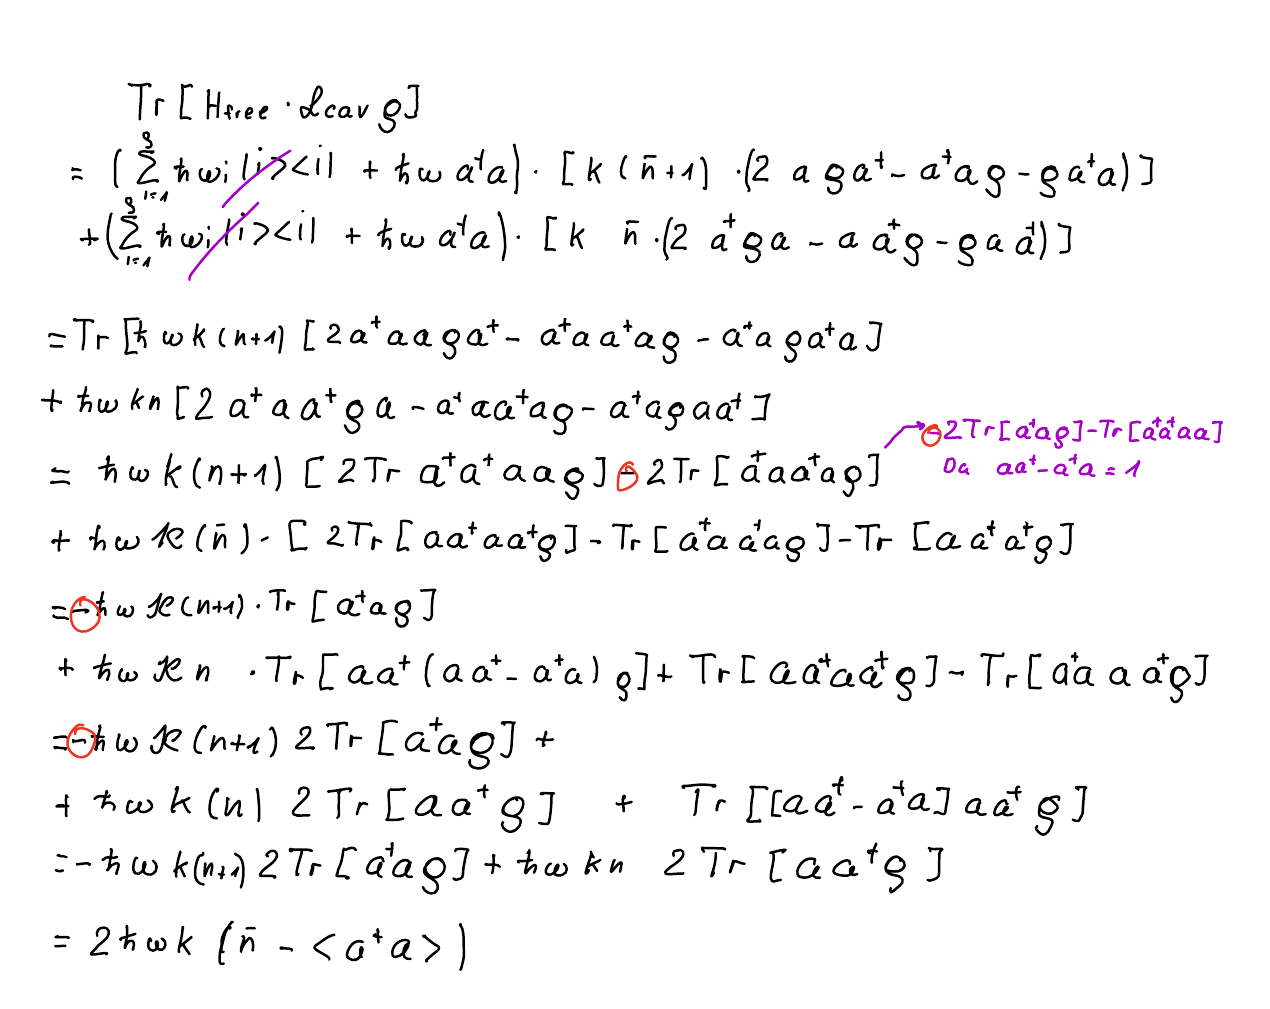
\includegraphics[scale=0.3]{Bilder-für-text/Berechnung-Tr[HL]2.png}
\caption{Calculation for $ Tr[H \mathcal{L}]$.}
\end{figure}

\subsection{Software}
For the implementation of the three-level-system in a cavity, I used qutip. Qutip is a python library, which allows to solving master equation fast.
Further calculations and methods were easily applied in python. 

\end{document}
Because,
in this regime, the system has already a population inversion
thus the increase of the hot bath temperature $T_h$
can no longer bring in a significant increase to the photons gain.
The hot bath no longer has
any weakening effect to the lasing, thus more lasing photons
can be produced in the cavity, and the lasing power can be
increased. But, still, the cavity photon number is limited due to
the single atom feature.%                                                                                               sander@sanders-arch ☺ ~/Sand